\chapter{Project Vision}
\label{ch:vision}

This chapter presents the vision behind AetherFlow. It describes the problem domain, states and elaborates the problem the project addresses, and sets out the goals, scope, constraints, and business opportunity of the work. It also identifies the stakeholders who benefit from the gateway. Together, these sections explain why a privacy-centric, multi-objective LLM gateway is needed and what the project aims to deliver.

%--------------------------------------------------------------
\section{Problem Domain Overview}
\label{sec:domain}

Large Language Models (LLMs) are now used in code assistants, chatbots, and corporate search. In an enterprise, these applications rarely depend on a single model. They draw on a mix of high-capability commercial cloud models and smaller open-weight models hosted on-premise, and each has different cost, speed, quality, and data-handling characteristics.

Without a mediation layer, a client application is usually connected to one provider. The organization is then forced into a choice. It can send all traffic to the strongest cloud models, which is costly, adds latency, and exposes prompts to external services. Or it can restrict users to local models, which keeps data on-premise but lowers output quality on difficult tasks. Neither choice uses the available models according to what each request actually needs.

AetherFlow addresses this problem as a gateway between clients and model backends. Figure~\ref{fig:overview} shows its position in the overall system.

\begin{figure}[htbp]
\centering
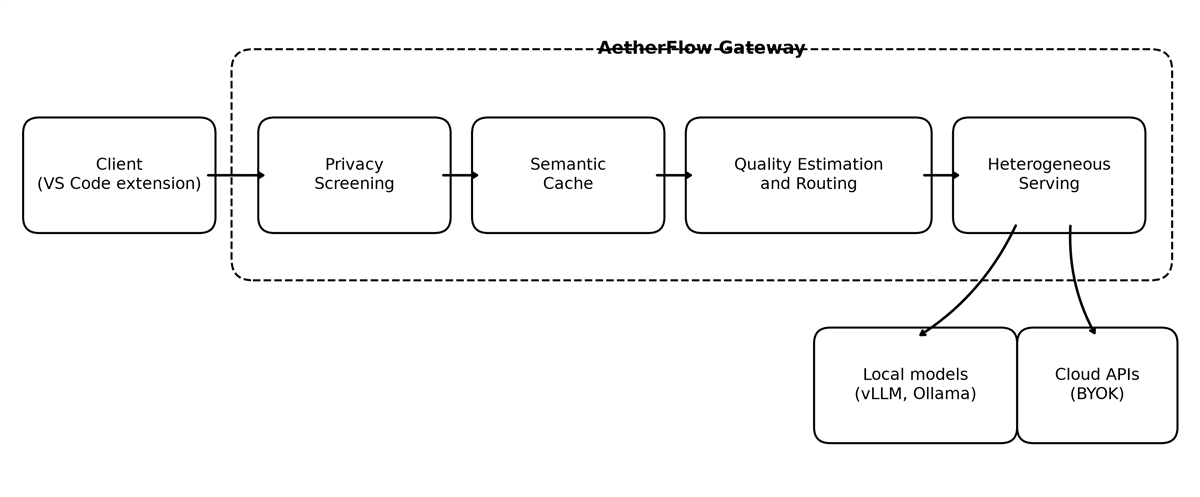
\includegraphics[width=0.98\textwidth]{Figures/overview.png}
\caption{Position of the AetherFlow gateway between client applications and model backends}
\label{fig:overview}
\end{figure}

%--------------------------------------------------------------
\section{Problem Statement}
\label{sec:problem-statement}

Organizations that use LLMs at scale need to decide, for each request, which model should handle it. A good decision must weigh output quality, monetary cost, and response latency, and it must never send sensitive content to an external provider. Existing routing and gateway tools do not make this decision jointly. They either apply a fixed policy or choose between two models on prompt complexity alone.

Formally, let $q$ be an incoming query and let $M = \{m_1, \dots, m_K\}$ be the set of registered backends, covering both local models and cloud models. For each pair $(q, m_k)$, let $\hat{Q}(q, m_k) \in [0,1]$ be the estimated quality of the response, $C(q, m_k) \ge 0$ the expected monetary cost, $L(m_k) \ge 0$ the current latency of the backend, and $P(q, m_k) \in \{0,1\}$ an indicator that is $1$ if sending $q$ to $m_k$ would violate a privacy policy. The goal of AetherFlow is to select the backend
\begin{equation}
m^{*} = \arg\max_{m_k \in M_{\mathrm{feasible}}} \; w_q\,\hat{Q}(q, m_k) \; - \; w_c\,\hat{C}(q, m_k) \; - \; w_l\,\hat{L}(m_k),
\label{eq:objective}
\end{equation}
where $M_{\mathrm{feasible}} = \{\, m_k \in M : P(q, m_k) = 0 \,\}$, the cost and latency terms are normalized, and $w_q, w_c, w_l \ge 0$ are administrator-defined weights with $w_q + w_c + w_l = 1$. Privacy is therefore applied as a hard constraint that removes unsafe backends before any trade-off is made, and it is not one of the weighted terms.

%--------------------------------------------------------------
\section{Problem Elaboration}
\label{sec:elaboration}

The problem statement above can be divided into the following sub-problems.

\subsection{Balancing Cost and Quality}
Cloud LLM providers charge per token, so costs grow with the number of requests. Many requests, such as formatting or routine refactoring, can be handled by a smaller local model, while others need the reasoning ability of a frontier model. When every request goes to the same model, the organization either overpays for simple tasks or loses quality on complex ones. A router therefore needs an estimate of how well a candidate model will answer a given prompt, before the prompt is executed.

\subsection{Latency Variability}
Interactive tools such as code assistants depend on fast responses. Requests to cloud APIs cross public networks and shared infrastructure, so response times can vary. Locally hosted models give more predictable latency but may be slower or weaker on some tasks. The router should therefore take current backend latency into account, and the gateway's own decision overhead must remain small.

\subsection{Privacy and Sensitive Data}
Prompts in software engineering workflows can contain personally identifiable information, credentials, or proprietary code, often unintentionally. Such data should not be passed to external providers, and regulations such as GDPR and HIPAA are a major reason why. The gateway should detect these categories of data before routing, mask them where appropriate, and keep confidential requests on local models.

\subsection{Limits of Static Routing}
Existing tools do not make a joint decision over all four requirements. LiteLLM offers a unified interface to multiple providers, but its routing is static. RouteLLM \cite{ref:RouteLLM} learns to choose between a stronger and a weaker model, but it considers only prompt complexity and not live latency, remaining budget, or data sensitivity. These tools are examined in detail in Chapter~3.

\subsection{Semantic Cache False Positives}
Caching responses for repeated queries can reduce both cost and latency. A semantic cache \cite{ref:GPTCache} matches new queries to earlier ones by embedding similarity rather than exact text. However, similarity alone can be unreliable: two prompts with opposite meanings, such as ``encrypt'' and ``decrypt'', can have very similar embeddings. Returning a cached answer in such a case would give the user an incorrect response. The cache must therefore verify that a candidate answer is appropriate before serving it.

%--------------------------------------------------------------
\section{Goals and Objectives}
\label{sec:goals}

The main goal of AetherFlow is to route each request by multi-objective decision making and not by fixed heuristics. The specific objectives are as follows:

\begin{enumerate}
    \item Deliver a multi-objective utility engine that selects the best routing target using a weighted function of quality, cost, and latency, under a privacy constraint.
    \item Enforce privacy-aware execution through query sensitivity analysis, PII masking, and local-only execution of confidential inputs.
    \item Minimize response latency, targeting under 200\,ms for cached queries and under 15\,ms of policy-engine decision overhead.
    \item Develop a semantic cache that checks the consistency of a candidate answer before serving it, in order to reduce false-positive cache hits.
    \item Provide an observability dashboard that reports cost savings, latency, cache hit ratio, and the real-time distribution of queries across models.
    \item Deliver a VS Code extension as the reference client, with a chat panel and code-aware actions (explain, fix, refactor, and generate tests) that call the gateway through its API.
\end{enumerate}

%--------------------------------------------------------------
\section{Project Scope}
\label{sec:scope}

The scope of this project is the development of the AetherFlow gateway as a stand-alone, asynchronous FastAPI proxy service. The gateway includes a Privacy Analyzer, a semantic cache, a multi-objective routing engine, and an observability dashboard. It routes between a live subset of local models (Qwen3-8B and Llama-3.1-8B-Instruct) and cloud APIs such as GPT and Gemini, accessed with user-supplied API keys (Bring Your Own Key). The reference client is a VS Code extension that offers a chat panel and code-aware actions on top of the gateway. The system is evaluated on public benchmarks (MMLU, GSM8K, HumanEval, and MT-Bench) and not in a live production environment.

The following are outside the scope of the project:

\begin{enumerate}
    \item Development of new language models.
    \item Construction of a general identity and access management service.
    \item Support for an open-ended number of third-party model providers.
\end{enumerate}

Support for additional providers, a confidence estimator for local models, and clients for other IDEs (for example, Cursor and JetBrains) are treated as stretch goals.

%--------------------------------------------------------------
\section{Sustainable Development Goal (SDG)}
\label{sec:sdg}

AetherFlow aligns with two United Nations Sustainable Development Goals, shown in Figure~\ref{fig:sdg}.

\begin{figure}[htbp]
\centering
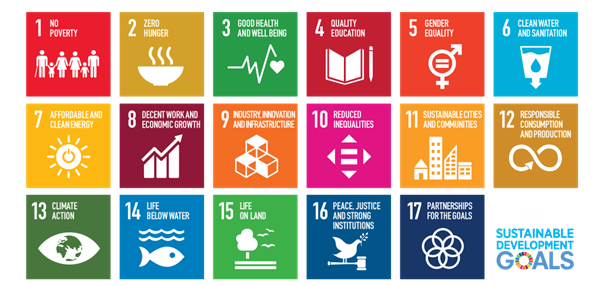
\includegraphics[width=0.75\textwidth]{Figures/Picture1.png}
\caption{Sustainable Development Goals targeted by AetherFlow: Goal 9 (Industry, Innovation, and Infrastructure) and Goal 12 (Responsible Consumption and Production)}
\label{fig:sdg}
\end{figure}

\begin{enumerate}
    \item SDG 9 (Industry, Innovation, and Infrastructure): AetherFlow supports innovation in digital infrastructure by helping organizations use generative AI through a mix of local and cloud models, so that access to advanced models does not depend on a single costly provider.
    \item SDG 12 (Responsible Consumption and Production): By sending routine requests to smaller local models and serving repeated queries from a cache, AetherFlow avoids unnecessary use of large cloud models and encourages more efficient use of computing resources.
\end{enumerate}

%--------------------------------------------------------------
\section{Constraints}
\label{sec:constraints}

The design and development of AetherFlow are subject to the following constraints:

\begin{enumerate}
    \item Hardware: The gateway and its supporting models (Presidio, the embedding and cross-encoder models, and the quality estimator) are intended to run within limited host memory, with or without GPU acceleration. The local language models are limited to the 8B-parameter class, which suits quantized on-premise serving.
    \item Cloud access: Cloud models are used through user-supplied API keys, so their availability, pricing, and rate limits are controlled by external providers.
    \item Offline operation: For confidential requests, the gateway must be able to operate without outbound internet access.
    \item Protocol compatibility: The gateway interface should follow a widely used API format, so that existing client tools can connect with little or no modification.
    \item Evaluation: Results are obtained from public benchmarks and a prepared corpus of model responses, and not from a live production deployment.
    \item Time and resources: The project is carried out within the schedule and resources of a Final Year Project.
\end{enumerate}

%--------------------------------------------------------------
\section{Business Opportunity}
\label{sec:business}

Organizations that adopt LLMs widely face rising API costs and growing concern about data protection. A gateway that lowers cloud spending by serving suitable requests locally or from a cache, and that keeps sensitive prompts inside the organization, addresses both concerns at once. Because AetherFlow works behind a simple API, it can be placed in front of existing tools without changing how developers work.

The same design can serve many kinds of applications and not only coding assistants. Teams that handle confidential data, such as software companies, financial institutions, and healthcare providers, are natural users. The observability dashboard also gives management visibility into usage and cost, which supports budgeting decisions on LLM adoption.

%--------------------------------------------------------------
\section{Stakeholders Description}
\label{sec:stakeholders}

\subsection{Stakeholders Summary}
\label{subsec:stakeholder-summary}

The main stakeholders of AetherFlow are as follows:

\begin{enumerate}
    \item Software developers are the primary users. They send requests through the VS Code extension and expect fast, accurate responses.
    \item System administrators deploy the gateway, manage model backends and API keys, configure routing weights, and monitor system health through the dashboard.
    \item Information security and compliance personnel review how sensitive data is detected, masked, and kept from external providers.
    \item Management and finance teams oversee the budget for LLM usage and use the dashboard to track cost savings and usage.
\end{enumerate}

\subsection{Key High-Level Goals and Problems of Stakeholders}
\label{subsec:stakeholder-goals}

Each stakeholder group has its own goals and concerns:

\begin{enumerate}
    \item Software developers want quick, high-quality responses without worrying about whether their prompts contain sensitive information.
    \item System administrators want a gateway that is simple to deploy, configure, and monitor.
    \item Information security and compliance personnel want assurance that confidential data does not leave the organization.
    \item Management and finance teams want predictable costs and clear visibility into how models are being used.
\end{enumerate}

%--------------------------------------------------------------
\section{Conclusion}
\label{sec:ch2-conclusion}

This chapter presented the vision of AetherFlow. It described the problem domain, stated the routing problem formally, and elaborated its main sub-problems: cost and quality balance, latency variability, privacy, the limits of static routing, and unreliable semantic caching. It then set out the objectives, scope, SDG alignment, constraints, business opportunity, and stakeholders of the project. The next chapter reviews related work and applications.


%% ============================================================
%%  CHAPTER 3: LITERATURE REVIEW AND RELATED APPLICATIONS
%% ============================================================
